\documentclass[a4paper,12pt]{article}

\usepackage{cmap}
\usepackage{type1ec}
\usepackage[T2A]{fontenc}
\usepackage[utf8]{inputenc}
\usepackage[english,russian]{babel}
\usepackage[margin=2.5cm]{geometry}
\usepackage{microtype}
\usepackage{amsmath,amssymb}
\usepackage{listings}
\usepackage{graphicx}

\usepackage[hidelinks,unicode]{hyperref}

\lstset{
    basicstyle=\ttfamily\small,
    breaklines=true,
    columns=fullflexible,
    keepspaces=true,
    showstringspaces=false,
    frame=single,
    framerule=0.3pt
}

\usepackage[most]{tcolorbox}
\newtcolorbox{ai}[1][]{
  colback=gray!5,      % Цвет фона (очень светлый серый)
  colframe=gray!70,    % Цвет рамки
  title={Текст сгенерированный ИИ},            % Заголовок, который будет отображаться
  fonttitle=\bfseries\sffamily, % Шрифт заголовка
  boxrule=0.5pt,       % Толщина линии рамки
  sharp corners,       % Прямые углы (можно убрать для скруглённых)
  breakable            % Позволяет рамке разрываться между страницами
}

% Короткая пометка внутри абзаца.
\newcommand{\term}[1]{\textbf{#1}}

% Вопрос, который ещё не закрыт.
\newcommand{\openq}[1]{\par\noindent\textit{Вопрос.} #1\par}

% Наблюдение по эксперименту или чтению.
\newcommand{\obs}[1]{\par\noindent\textit{Наблюдение.} #1\par}

\title{Cache-Conscious Structure Definition}
\author{Олег Шипулин}
\date{\today}

\begin{document}

\maketitle
\tableofcontents
\newpage


\section{Постановка}

\subsection{Кратко о задаче}

\hspace{0.5 cm} Сторона кода в PGO изучена хорошо, сторона данных почти нет. Цель проекта: инструмент, который по аппаратным профилям обращений к памяти (PEBS или аналог) автоматически:

\begin{itemize}
    \item разделяет горячие и холодные поля структур;
    \item переупорядочивает члены структур;
    \item меняет размещение объектов при выделении памяти,
\end{itemize}

чтобы working set занимал меньше кеш-линий и страниц.

\subsection{Контекст}

\hspace{0.5 cm} PGO, BOLT и Propeller переставляют код: функции, базовые блоки, горячие/холодные части. Data layout при этом остаётся таким, каким его написал программист. 

Порядок полей определяется читаемостью, а не частотой обращений, а горячие и холодные объекты одного типа лежат вперемешку. При этом механизмы аппаратного сэмплирования (Intel PEBS, AMD IBS) умеют давать адреса обращений к данным, то есть исходные данные для такой оптимизации есть.

\subsection{Исследовательская сложность}

\begin{itemize}
    \item Профиль выборочный и неполный: часть полей и объектов в нём просто не встретится.
    \item Язык позволяет брать адреса данных, есть offsetof, касты, сериализация через memcpy, ограничения ABI. Поэтому нужно доказывать, что преобразование безопасно, а не просто выгодно.
    \item Нужно подтвердить, что перезапись сохраняет семантику программы.
\end{itemize}

\subsection{Возможный план}

\begin{enumerate}
    \item Изучить предшествующие попытки, прежде всего GCC -fipa-struct-reorg и -fipa-reorder-fields, и разобраться, почему struct-reorg из GCC убрали: какие проблемы безопасности или поддержки не удалось решить.
    \item Собрать профили обращений к памяти (perf mem, perf c2c, PEBS/IBS) и сопоставить адреса с полями структур через отладочную информацию.
    \item Определить класс безопасных преобразований и анализ, который их
        разрешает: escape analysis, отсутствие взятия адреса, отсутствие внешней
        видимости типа.
    \item Реализовать преобразования: переупорядочивание полей, hot/cold splitting структур, раздельные арены для горячих и холодных аллокаций. Здесь стоит опереться на существующие hot/cold hints для аллокаторов: operator new с hot/cold hint в tcmalloc и LLVM MemProf, который расставляет такие hints по профилю.
    \item Измерить эффект: cache-miss, TLB-miss, задержка/пропускная способность на реальных нагрузках.
\end{enumerate}


\subsection{Ожидаемый результат:}

\begin{itemize}
    \item Инструмент: профиль → рекомендации или автоматическое преобразование кода (на уровне компилятора или исходников).
    \item Анализ безопасности преобразований и его ограничения.
    \item Измерения на нескольких программах.
\end{itemize}


\subsection{С чего начать:}
\begin{itemize}
    \item Chilimbi, Davidson, Larus. Cache-conscious structure definition (PLDI 1999) и смежные работы по cache-conscious layout.
    \item GCC -fipa-struct-reorg, -fipa-reorder-fields и история их удаления.
    \item LLVM MemProf, hot/cold hints в tcmalloc.
    \item Документация Intel PEBS / AMD IBS, perf mem, perf c2c.
\end{itemize}

\subsection{Мой более подробный план:}

\hspace{0.5 cm} Так как сфера мне целиком не известна, я собираюсь изучить
целиком материал о том, как теоретически могут быть написаны эти оптимизации,
как они уже реализовывались и почему не получились. Однако необходимо
продумать, как сохранить семантическую корректность и целостность, а также
доказать эффективность. Для этого я расписал план изучения на следующее время.

После каждой фазы необходимо выписать какие-то определенные критерии прохождения
этого этапа.
\subsubsection{Фаза 0. Постановка}

Сначала необходимо узнать, уже придуманные приёмы и почему они не получились.

\begin{itemize}
    \item
        \href{https://sourceforge.net/projects/cpp-lects-rus/files/cpp-graduate/16-llvm.pdf/download}{Константин
        Владимиров: LLVM.} --- Основы LLVM и экосистема, Генерация IR, RTTI в стиле 
        LLVM, Оптимизации в LLVM.

    \item Chilimbi, Davidson, Larus. \textit{Cache-Conscious
    Structure Definition}. \\
    PLDI 1999. Reorder и splitting по профилю. Граф
    близости полей: вместе класть то, к чему обращаются рядом по
    времени, а не просто самые частые поля.
    \item Chilimbi, Hill, Larus. \textit{Cache-Conscious Structure
    Layout}. PLDI 1999. Размещение самих объектов в куче.
    \item LLVM MemProf, \url{https://llvm.org/docs/MemProf.html}.
    Готовый сбор профиля аллокаций и hot/cold hints. 
    \item GCC \texttt{-fipa-struct-reorg} и
    \texttt{-fipa-reorder-fields}: что проход умел и почему
    \texttt{-fipa-struct-reorg} убрали. Какие отказы по безопасности
    и сопровождению так и не закрыли. 
    \item Hundt, Mannarswamy, Chakrabarti. \textit{Practical Structure
    Layout Optimization and Advice}. CGO 2006. 
\end{itemize}

Результат фазы: понимание существующих подходов, а также их проблемы реализации
с gcc. Фаза будет являться вступлением для того, чтобы осознать общую задачу и проблему.

\subsubsection{Фаза 0.5. Baseline}

Необходимо определить baseline и критерии успешности проекта. 

\subsubsection{Фаза 1. Профиль обращений}

Так как для анализа необходимо собрать профиль обращений к памяти, нужно
определить, к какой конкретно архитектуре будет обращение. В зависимости от
этого нужно прочесть для Intel - PEBS, а для AMD --- IBS.

\begin{ai}
\begin{itemize}
    \item Intel: Intel SDM, Volume 3, глава Performance Monitoring.
    Формат PEBS-записи и memory-load facility: data linear address,
    latency, data source. Andi Kleen,
    заметки по PEBS и \url{https://github.com/andikleen/pmu-tools}:
    как из сэмпла достать IP и адрес данных.
    \item AMD: раздел IBS в документации процессора и то, как
    \texttt{perf} отдаёт data linear address для load и store.
    \item \texttt{man perf-mem} и
    \url{https://perf.wiki.kernel.org/} по \texttt{perf mem} и
    \texttt{mem-loads}. Команда одна и та же, источник сэмпла
    выбирает ядро.
    \item Что показывате perf c2c и пригодится ли он в работе
\end{itemize}
\end{ai}


Результат фазы: Научиться брать семплирование, а также отвечать на вопрос: какое
средство сэмплирования необходимо использовать для нашей задачи и в каком
случае. 

\subsubsection{Фаза 2. От адреса к полю}

После получения адресов, необходимо осознать, как адрес из профиля можно
превратить в поле. Далее нагенеренное чтиво, по которому необходимо разобраться: 


\begin{ai}
\begin{itemize}
    \item В DWARF беру тег члена, его смещение и location lists. \\
    Тег называется \texttt{DW\_TAG\_member}. Дамп смотрю командой
    \texttt{llvm-dwarfdump}.
    \item LLVM, Source Level Debugging:
    \url{https://llvm.org/docs/SourceLevelDebugging.html}.
    В IR имя поля лежит в debug info, не в типе инструкции.
    \item \texttt{DataLayout} в LLVM: размеры типов, alignment и
    endianness для x86-64. По ним смещение в байтах становится
    конкретным полем.
\end{itemize}

Два разных случая.

\begin{itemize}
    \item Глобал: символ плюс смещение, дальше запись поля в DWARF.
    \item Куча: база объекта из сэмпла неизвестна. Нужен перехват
    аллокации с типом (обёртка аллокатора или пометка в Clang).
    Иначе адрес не к чему привязать. Стек и location lists --- после
    кучи и глобалов.
\end{itemize}

Дальше считаю частоту поля и совместный доступ: граф близости из
фазы 0.

Clang опускает поле в смещение двумя конструкциями IR.
Сначала \texttt{StructType}, затем \texttt{getelementptr}.
После SROA и mem2reg
структура часто уже разобрана на скаляры, поэтому имя поля в
инструкции не остаётся: оно живёт в debug info и в AST. Полный курс
SSA к таблице полей не нужен. Справочник по конкретной инструкции
LLVM открываю по ходу, Language Reference целиком не читаю.

\end{ai}

Результат фазы, который можно определить таблицей в формате:

\begin{itemize}
    \item тип,
    \item поле, 
    \item число обращений,
    \item какие cache line задеты.
\end{itemize}

... (Как уменьшить отступы между элементами в списке latex) ...

\subsubsection{Фаза 3. Безопасные преобразования}

Проблема преобразований стоит явно, ведь непонятно, как доказать их корректность
после оптимизаций. 

\begin{ai}

\begin{itemize}
    \item System V AMD64 ABI, раздел про aggregates: alignment,
    padding, как структуру передают в вызов.
    \item Itanium C++ ABI, глава 2. Clang на Linux кладёт объекты по
    ней: vptr, базы, виртуальные базы. vptr остаётся в начале
    объекта.
    \item Hagog, Tice. \textit{Cache Aware Data Layout Reorganization
    Optimization in GCC}. GCC Summit 2005. Когда reorder и split
    запрещены: address-taken, \texttt{volatile}, внешний ABI,
    битовые поля, union. Это разбор того, что в фазе 0 осталось
    списком отказов GCC.
\end{itemize}

Анализ, который разрешает преобразование, --- escape analysis:
адрес поля не уходит из модуля, тип не виден снаружи. Alias analysis
LLVM открываю только на этот вопрос. TBAA отвечает за strict
aliasing, к горячим и холодным полям он не относится. Вывод Hundt из
фазы 0 применяю к конкретному типу: публичный тип остаётся
рекомендацией.

Раскладку C++-структуры задаёт Clang, поэтому к типу иду через AST.
Нужные узлы --- \texttt{RecordDecl} и \texttt{FieldDecl}. Это ближе к задаче, чем
переписывание \texttt{getelementptr} в середине пайплайна.
Перестановка полей объекта --- решение фронтенда и ABI.

Тип не трогаю, если он в публичном заголовке, объявлен
\texttt{extern "C"}, адрес поля сохраняется, наружу торчит
\texttt{offsetof}, есть union, каст или сериализация всего объекта
через \texttt{memcpy}.

\end{ai}

Результат фазы: класс безопасных преобразований и его границы.
Чеклист отказа на одном своём типе. Тип, который чеклист пропускает,
идёт в фазу 4.

\subsubsection{Фаза 4. Носитель инструмента}

Выбираю, где живёт преобразование, и дочитываю только этот кусок
LLVM. Носители от простого к сложному.

\begin{ai}
\begin{enumerate}
    \item Отчёт: рекомендованный порядок полей и split, правки
    руками. На нём видно, безопасно ли преобразование.
    \item Clang-плагин на \texttt{RecordDecl} и \texttt{FieldDecl},
    при необходимости \texttt{Rewriter}. Для типов с internal
    linkage, поля которых не address-taken.
    \item LLVM-pass для структур, которые не убегают наружу. Тогда
    уже нужны IR памяти (\texttt{load}, \texttt{store},
    \texttt{getelementptr}, \texttt{StructType}), запуск через
    \texttt{opt} или \texttt{clang -fpass-plugin}, различие analysis
    pass и transform pass. Подсчёт \texttt{load} и \texttt{store}
    профиль памяти не заменяет: это только способ убедиться, что
    плагин запускается. Книги LLVM Essentials и Getting Started with
    LLVM Core Libraries не беру: API там старый. Новый Pass Manager
    описан в Writing an LLVM Pass,
    \url{https://llvm.org/docs/WritingAnLLVMNewPMPass.html}.
\end{enumerate}

Проход компилятора пишу, если отчёта и правки AST мало.

Placement объектов делаю через hot/cold hint на аллокацию: LLVM
MemProf и \texttt{operator new} с hot/cold в tcmalloc. Hint помечает
объект целиком, не поле, поэтому reorder и split им не заменяются.
Свой аллокатор или арена --- если hint не раскладывает горячие и
холодные объекты по разным областям. Pass для placement не нужен.

Порядок внутри фазы: сначала reorder с тем же alignment и тестом,
что значения на выходе совпали. Split вторым. Placement третьим.
\end{ai}

Результат фазы: одно преобразование на одном закрытом типе,
программа считает то же самое.

\subsubsection{Фаза 5. Измерения}

\begin{ai}
Ответ по задаче --- влияние на cache misses, working set и latency.

До первого прогона читаю Mytkowicz et al. \textit{Producing Wrong
Data Without Doing Anything Obviously Wrong!} ASPLOS 2009.

Снимаю:

\begin{itemize}
    \item \texttt{mem\_load\_retired.*}, \texttt{LLC-load-misses},
    \texttt{dTLB-load-misses};
    \item сколько cache line и страниц трогает горячий путь;
    \item latency участка гистограммой и пропускную способность того
    же прогона.
\end{itemize}

Рядом контроль: значения на выходе совпали. Один и тот же workload,
зафиксированные CPU и частота.

Результат фазы: одна таблица до и после на одной программе и список
того, что инструмент не стал менять (address-taken, низкая
уверенность профиля, ABI).

Следующий замер --- несколько программ и реальная нагрузка. Его
начинаю после этой таблицы: адрес уже стал полем, одно
преобразование уже посчитано.
\end{ai}


\section{Первый шаг: Прочтение литературы}

Для того, чтобы понять цель задачи, необходимо вникнуть в материал, потому что
прошлого опыта работы в данной сфере не было. Самые известные работы:

\begin{itemize}
    \item
        \href{https://sourceforge.net/projects/cpp-lects-rus/files/cpp-graduate/16-llvm.pdf/download}{Константин
        Владимиров: LLVM.} --- Основы LLVM и экосистема, Генерация IR, RTTI в стиле 
        LLVM, Оптимизации в LLVM.

    \item Chilimbi, Davidson, Larus. \textit{Cache-Conscious
    Structure Definition}. \\
    PLDI 1999. Reorder и splitting по профилю. Граф
    близости полей: вместе класть то, к чему обращаются рядом по
    времени, а не просто самые частые поля.
    \item Chilimbi, Hill, Larus. \textit{Cache-Conscious Structure
    Layout}. PLDI 1999. Размещение самих объектов в куче.
    \item LLVM MemProf, \url{https://llvm.org/docs/MemProf.html}.
    Готовый сбор профиля аллокаций и hot/cold hints. 
    \item GCC \texttt{-fipa-struct-reorg} и
    \texttt{-fipa-reorder-fields}: что проход умел и почему
    \texttt{-fipa-struct-reorg} убрали. Какие отказы по безопасности
    и сопровождению так и не закрыли. 
    \item Hundt, Mannarswamy, Chakrabarti. \textit{Practical Structure
    Layout Optimization and Advice}. CGO 2006. 
\end{itemize}

Так как материала достаточно много, я принял решение потратить дополнительное
время и конспектировать основные идеи из каждого учения.

\subsection{Константин Владимиров: LLVM}


В контексте проекта интереснее всего смотреть за работу с памятью. Всё
происходит через store/load по указателю (то есть все переменные хранят не само 
значение, а указатель). Кроме того, каждое изменение переменное порождает новую
переменную. Память в LLVM — это просто плоский массив байт. Нельзя сказать "дай
мне значение переменной x". Можно только сказать "загрузи значение по адресу, 
который лежит в указателе \%ptr" (инструкция load). Именно поэтому getelementptr 
нужен, так как он вычисляет эти адреса.

Из-за этого можно анализировать GEP инструкции в купе со store/load 
в LLVM для нахождения hot/cold частей структур. 

Отдельное важное уточнение - \textbf{alloca}.
\begin{lstlisting}
    %ptr = alloca i32, align 4
\end{lstlisting}

Живет на стеке. Можно перезаписывать через store. Медленнее, но позволяет брать
адрес и менять значение. Это важно, потому что \textbf{текущий проект} анализирует 
memory access patterns. alloca — это источник указателей для большинства load/store.

Если есть код:
\begin{lstlisting}
%ptr = alloca %struct.S
%field = getelementptr %struct.S, %struct.S* %ptr, i32 0, i32 2
store float 1.0, float* %field
\end{lstlisting}

То понятно, что это локальная структура на стеке, и мы пишем в её третье поле. Такие
обращения очень быстрые (стек горячий), но они всё равно занимают cache lines.
Если структура большая, а используется только одно поле — это проблема.

В LLVM есть отдельная оптимизация - mem2reg, который удаляет alloca, если может доказать,
что:

\begin{itemize}
    \item Адрес переменной не уходит за пределы функции.
    \item Нет сложного алиасинга.
\end{itemize}

После mem2reg все load/store заменяются на SSA-значения и phi-узлы. Если нужно анализировать
IR, то это необходимо до mem2reg (или отключать его), потому что именно там видны реальные обращения к памяти. После mem2reg от структуры данных останутся только абстрактные регистры,
и нельзя будет понять, какие поля были горячими.

Последний важный пункт, который я хотел бы подчеркнуть из лекции - оптимизации в
LLVM. LLVM 11 делает более 100 высокоуровневых оптимизаций. Это огромное
количество. Каждая оптимизация — это отдельный проход, который преобразует IR.
Эти оптимизации называются \textbf{Pass Pipeline}. Благодаря определенным
параметрам можно посмотреть иерархически, какие оптимизации когда применяются, а
также посмотреть IR до конкретной оптимизации и после.

\subsubsection{Вывод для проекта:}

\begin{itemize}
    \item Для анализа вручную горячих мест, если понадобится, необходимо исследовать 
        alloca, store, load. 
    \item Мой проход должен входить в LLVM иерархию и быть зарегистрированным через 
        -fpass-plugin.
    \item Надо отчетливо понимать, где конкретно в конвейере должна быть моя
        оптимизация.
\end{itemize}

\subsection{Cache-Conscious Structure Definition}

Данное учение является центральным для данного проекта, потому что рассказывает
непосредственно о том, как данные внутри структур можно разбивать. Есть
несколько основных подходов:

\begin{enumerate}
    \item structure splitting;
    \item field reordering.
\end{enumerate}

Надо понимать, что данная статья является продолжением изучения темы об
улучшении производительности, где были исследованы методы оптимизацию кэша за счет
изменения расположения отдельных экземпляров структур в памяти, а не их внутреннего
устройства. Ключевая идея этих методов — co-location, где объекты пытаются
разместить в одном кэш-блоке, если они часто используются вместо. Это статья
считается продолжением этих исследований, но для больших объектов, где нельзя
просто взять и разместить несколько объектов в одном кэше, потому что размеры
кэша ограничены.


\textbf{\textit{Общая идея:}}

Мы рассматриваем, как можно переупорядочить содержимое структуры так, чтобы
больше полезных данных попадало в кэш для уменьшения cache-misses.

\begin{figure}[h]
    \centering
    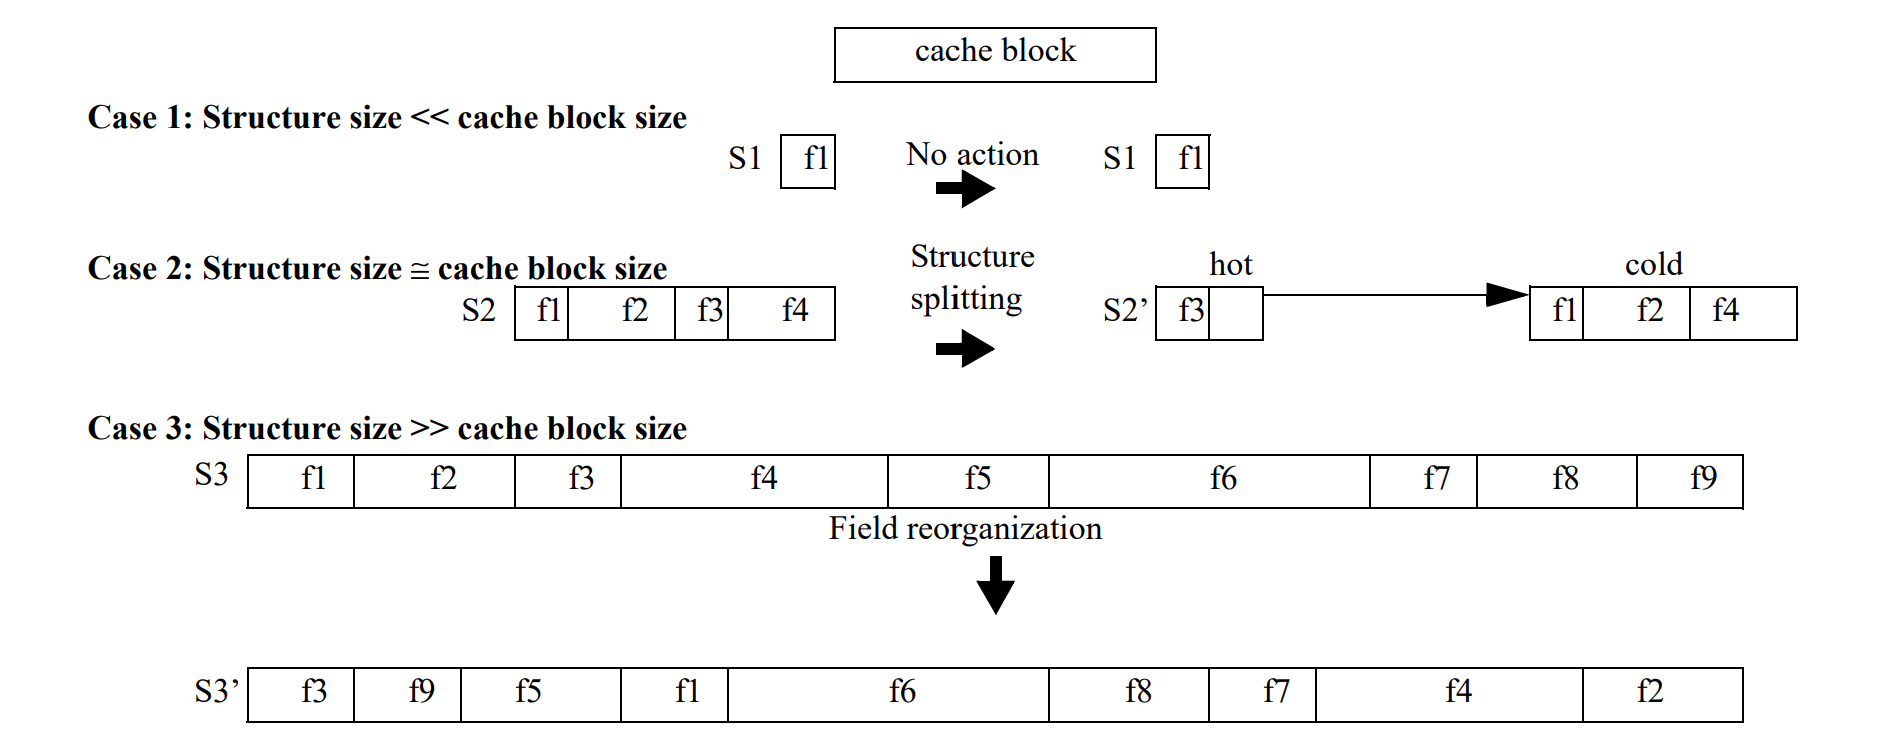
\includegraphics[width=0.8\textwidth]{./img/cache-conscious-struct-def.png}
    \caption{cache conscious struct definition}
\end{figure}

\subsubsection{Метод Splitting}

Один из способов splitting - разделить класс на hot и cold части, основываясь на
профилировании, а именно - как часто обращались к полям в классе. Благодаря
splitting можно поместить больше hot частей в cache block. 

Сразу с \textbf{проблем:} дополнительный указатель (занимает место), более медленный cold
path, расширение кода, больше объектов в памяти и т.д.. Кроме того, при не
репрезентативной входной нагрузке результаты могут быть искажены. 

Идея splitting'а применяется к классам, обращение к котором происходит
достаточно часто, из-за чего придумана формула:
\[
    A_i = \frac{LS}{100 * C}
\]
Где:
\begin{enumerate}
    \item LS — общее количество обращений к полям во всей программе;
    \item C — общее количество классов, к полям которых была хоть одна попытка
        обращения;
    \item $$A_i$$ — общее количество обращений к полям конкретного класса i;
\end{enumerate}

Таким образом, класс должен набрать хотя бы 1\% от среднего количества обращений по всем 
классам, чтобы считаться важным. Также класс должен иметь хотя бы 2 поля и быть
больше 8 байт.

После чего необходимо разделить класс на Hot и Cold части, используя \textbf{Агрессивный 
подход}:
\begin{enumerate}
    \item Правило: Поле помечается как «холодное», если к нему обращались не чаще, чем 
        $\frac{A_i}{2 * F_i}$ раз. 
        \begin{itemize}
            \item $F_i$ - количество полей в классе i. (То есть, если к полю обращаются в
                            два раза реже среднего по классу, оно отправляется в холод).
        \end{itemize}
    \item Проверка целесообразности: После этого алгоритм проверяет, достаточно ли велика
        получилась холодная часть. Она должна быть не менее 8 байт, чтобы окупить 
        затраты на создание и хранение ссылки на нее.
    \item Уравновешивание слишком агрессивного разделения: так как агрессивный
        подход может навредить в случае, если мы слишком много данных отправили
        в cold часть, и теперь приходится часто ходить по ссылкам, вводится формула:
        \[
            \frac{\max(hot(class_i)) - 2 * \Sigma cold(class_i)}{\max(hot(class_i))} > 0.5
        \]
        , где:
        \begin{itemize}
            \item max(hot) — количество обращений к самому горячему полю.
            \item $\Sigma$ cold — сумма обращений ко всем холодным полям.
        \end{itemize}
\end{enumerate}


\textbf{Реализация в Vortex:}
Чуваки запатчили Vortex компилятор и:
\begin{enumerate}
    \item \textit{Создали Cold Path.} Все поля, которые были помечены как "COLD"
        вырезаются из исходного класса, для которых создался еще один класс
        "PREVNAME\_OLD". Учитывается, что новый класс наследуется только от
        базового класса OBJECT и не содержит никаких методов, кроме
        конструктора. В новые класс был добавлен указатель на COLD Path
    \item \textit{Изменение горячего класса.} Так как в классе могли быть
        private и Protected поля, то их нельзя просто вырезать. Таким образом
        они были перенесены в другой класс с видимостью public. Таким 
    \item \textit{Изменение обращения кода к переменным.} Если было обращение к
        COLD path, то компилятор превращает это в HOT.COLD.field путь, то есть
        делая двойную косвенность. Также конструктор горячего класса должен в
        первую очередь создавать объект холодного класса.
\end{enumerate}

\textit{Проблемы в подходе:}
\begin{enumerate}
    \item Для проблемы с сериализацией надо оценить прирост производительности.
        Если он достаточен, то можно явно делать конвертер.
\end{enumerate}

\subsubsection{Метод reordering}
Идея - переставить внутри объекта поля местами, чтобы поля, которые используются
вместе, лежали рядом. Для этого используется \textbf{bbcache}. Он дает
рекомендации на основе профилирования, где пишет, какие поля стоит ставить друг
с другом. Он собирает данные в профилировании, потом смотрит на структуру
AST-дерева, объединяет информацию и говорит рекомендацию. Также даёт
метрики по локальности и количеству кэш блоков.

\begin{figure}[h]
    \centering
    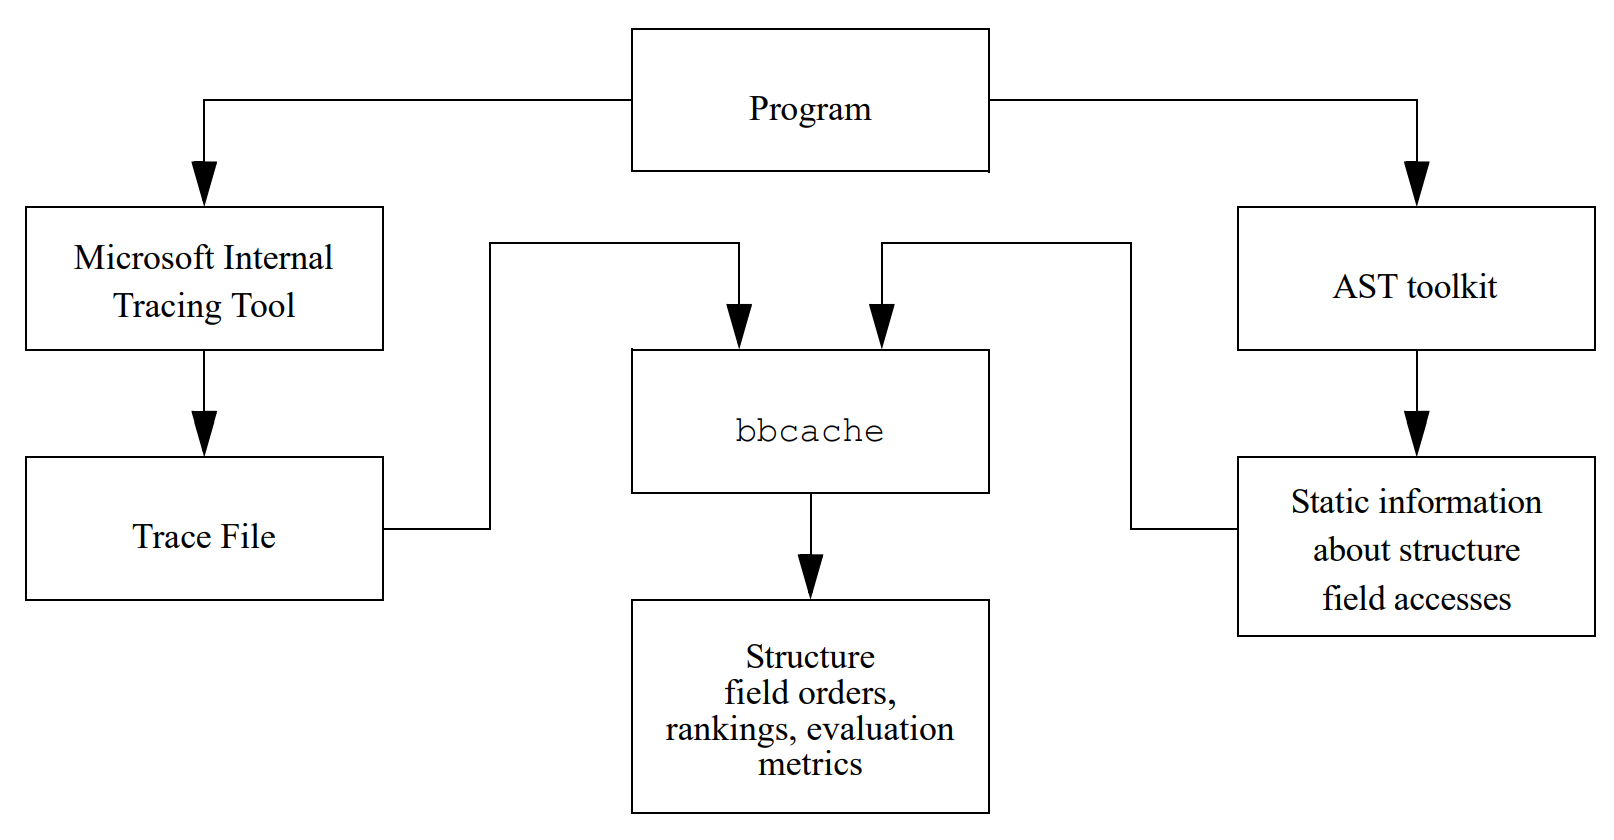
\includegraphics[width=0.8\textwidth]{./img/field_reodreing.png}
    \caption{field reodreing.png}
\end{figure}

\subsection{Попытки в GCC}
\subsubsection{-fipa-struct-reorg}




\subsection{Отчет}
1. Найти проект. 
2. GCC, про эти опции и почему выпилили подробно.

\end{document}
